\documentclass[12pt]{article}
\usepackage{geometry}                % See geometry.pdf to learn the layout options. There are lots.
\geometry{a4paper}                   % ... or a4paper or a5paper or ... 
%\geometry{landscape}                % Activate for for rotated page geometry
\usepackage[parfill]{parskip}    % Activate to begin paragraphs with an empty line rather than an indent
\usepackage{graphicx}
\usepackage{amssymb}
\usepackage{epstopdf}
\usepackage{color}
\usepackage{url}
\usepackage{helvet} %To the untrained eye helvetica and arial are pretty much identical
\renewcommand{\familydefault}{\sfdefault}

\DeclareGraphicsRule{.tif}{png}{.png}{`convert #1 `dirname #1`/`basename #1 .tif`.png}

\title{Near-field identities}
\author{TEAM NAME\\Alan Saul, Toby Gilham, Jonathan Poulter}
\date{}                                           % Activate to display a given date or no date

\begin{document}
\maketitle
\newpage
\section{Summary}
{\color{red}{Executive summary of not more than one page, which summarises the content of the report.}}

Uses of short-range communication have been on the rise recently with many new technologies being established; such as Bluetooth, RFID and NFC. These innovations have allowed many new applications within near field identities, including ePassports, electronic identity cards and so-called e-money transactions. The introduction of ePassports has become a major concern to many security experts. Although their encryption methods (3DES, SHA-1, SHA-2 etc.) have been proven in many other security areas, some of the techniques for initiating conversations and verifying authenticity of electronic identities are flawed.

Luckily these vulnerabilities have not gone unnoticed. Protection from many of the threats such as skimming, forgery and unauthorised access are being constantly updated, by encompassing some the most advanced security techniques. 
This report will delve into the current technology being utilised to protect your electronic identity held within your ePassport. Initially we will discuss the idea of near field identities, and their social implications, we will then further focus on the ePassport technology and the protection that is embedded within. We will provide an overview of some of the classical encryption methods used, and compare authentication protocols that are being continually updated by many European countries since the introduction of ePassport technology. Further we will look at cases where vulnerabilities have been uncovered and how newly proposed techniques resolve the obsolete protocol's vulnerabilities.

\section{Introduction}
{\color{red}{Introduce the idea of near field identities, where they are likely to lead 
TODO}}

\section{Relevance}
Why is this material relevant to the security landscape now?
With the upcoming technology of ePassports being enforced within many countries including the UK, and the biometric data that will soon be held within, it is important to review what effects security breaches could have on unsuspecting victims.

The introduction of ePassports began in Malaysia in March 1998, actually predating the internationally accepted standard \cite{Avoine:2008wf}. ePassports have now become compulsory within many countries, including the vast majority of EU countries. The concern of aviation security spiked after the attacks of 9/11. Passports and visas are just one security aspect that was due an overhaul.

However not everyone has welcomed the introduction of electronic identities. Many privacy activists have voiced their concern over the invasion of privacy brought about by collecting personal data and storing it electronically \cite{Blundo:2008vs}. This has been particularly brought on by governments discussing the possibility of storing more sensitive biometric data within electronic identities, including fingerprint scans and iris scans. Indeed some governments, including Germany \cite{JRC:2008ws}, have begun compiling a centralised database of this biometric data. If this database was breached, the repercussions on the privacy of the individuals could be enormous. 

Gaining an understanding of the technologies currently in use, and standards that are being proposed for adding additional security layers is important if we wish to maintain our privacy, as we shall shortly see, the standards which are currently being used have been shown to possess a variety of security failures. Since ePassports are already being issued, securing these failures is an important requirement before more sensitive biometric data is additionally stored. Currently adult passports in the UK do not expire for 10 years following their issuance. Advances in computer forensics are likely to continue to sore in this period, it is important therefore to iron out potential pitfalls in the security of these systems if they are to stand a chance against the hackers of 2022. 

\section{Technical background}
{\color{red}{This section could cover the history of the topic, the mathematical background, or even the political context.
Prior to ePassports security}}

\subsection{RFID}
\label{sec:RFID}
Almost every countries producing ePassport's are building them around a data communication technology known as Radio Frequency Identification (RFID). This type of technology, often known as a ``tag" \cite{Juels:2005wf}, transmits its data wirelessly. The International Civil Aviation Organisation (ICAO) specifies a specific standard that must be met by all RFID tags used as ePassport chips (ISO 14443). 

RFID tags can come in two major forms, passive or active. The difference between the two forms is primarily the source of energy that consumes in order to carry out data transfers. An active RFID tag has an internal power source that powers the transmission of data. These are generally more expensive than their passive counterpart, last for a shorter length of time, and can transmit their data are longer distance.

The ISO 14443 standard is a passive RFID. This means that the chip has no internal source of power and should use power supplied by a reader interacting with the chip. Typically passive RFID tags can transmit up to 40ft however the ISO 14443 is typically designed to transmit only 10cm. This is by design, the shorter the distance the ePassport can be read at, the closer a potential attacker needs to be to the physical chip to interact with it. Many researchers have published results of eavesdropping on an existing transmission from up to 30ft, and initiating a transmission from 1.3ft \cite{Kfir:2005tv,Yoshida:2004ta} with modified card readers readily available from online shops.

An alternative technology for data transmission, and perhaps more appropriate for high stake security situations such as transmission of sensitive biometric data is contact chips. Contact chips, similarly to your chip and pin chip, require the reader to be in contact with the chip. This effectively removes two of the largest concerns with the use of RFID tags, the ability to eavesdrop on an existing communication, and the ability to skim information from the chip by passing close by it.

\subsection{Hashing?}
\label{sec:hashing}
{\color{red}{SHA-1/SHA-2 or refer to the other paper for reference to MD5?}}

\subsection{Public Key Infrastructure (PKI)}
\label{sec:PKI}
Digital signatures provide certification that a trusted third party believes someone's information to be correct. The document is signed by the private key of the sender, and decrypted using the public key of the sender that has been provided to the receiver. If when decrypted the document is illegible, the public key does not match the private key, thus the either the recipient has the wrong public key, or it was not signed by the private key of the expected sender. If it is legible you can be certain that the signature has not been lifted off another digital document.

Digital certificates go one step further than this. A third party can sign a document saying that they believe the information within is true. The details are summarised using a hashing function to provide a checksum of the information. The provided information can be verified to be the information that was signed by the third party by simply computing the hash of the information and confirming it matches the hash of the information that was signed.

Public Key Infrastructures (PKI's) serve as a method of managing, distributing and revoking digital certificates. PKI's have at least one Certification Authority (CA), these are trusted people or organisations that vouch for someone credibility. The CA will be in possession of their own public and private key pair, the private key should never be in the possession of another party as this is the tool used to sign certificates. When a certificate is requested from a CA by another party the CA will check that the party is who they say they are, and all information they are signing within the certificate is correct. The public key of the party requesting a certificate will be signed alongside the extra information they have provided so as to ensure that the certificate is directly related to a single body. An expiration date is usually associated with the certificate; the CA determines the length of validity of such certificates. PKI's can be hierarchical or distributed. In the hierarchical PKI's often multiple levels will exist. The CA's at the top of the hierarchy are called Root CA's. Parties in possession of a certificate may sign certificates for parties lower down in the tree, however they usually cannot permit activity that they themselves do not possess.

\section{3DES}
\label{sec:3DES}
{\color{red}{How 3DES works and how is it so secure (not the main thing to worry about in the overall system)}}
Triple Data Encryption Algorithm (3DES) is an implementation of the Data Encryption Standard (DES) cipher algorithm three times to each data block we'll go over the basics of DES to help explain 3DES
\subsection{DES}


\section{Structure of ePassport}
\label{sec:LDS}
One of the main purposes of an ePassport is providing proof of identity when entering a new country. In order to do this an agreed structure of information and protocols need to be internationally standardized and agreed on. ICAO has set the standardized Logical Data Structure (LDS) that is widely used by countries implementing ePassport technology (Figure~\ref{fig:LDS}).

The data structure currently contains 16 Data Groups, soon to be 18, denoted DG1-DG18 respectively. Many of these Data Groups are not mandatory to conform to ICAO standards, however DG1 (All information printed on the Machine Readable Zone (MRZ) of the passport - basic personal information including name, DOB, passport number etc.) and DG2 (encoded biometric image of the face) are \cite{Anonymous:2006vu}. As of 2009 the presence of DG3-DG14 (including fingerprint scans, and iris images and additional personal details such as telephone number, proof of citizenship and custody information) have become a mandatory for EU countries \cite{Anonymous:2011vj}. However the presence of these data groups does not enforce that they are completed.

More interestingly for a cryptologist additional files containing digital signatures of the data groups is mandatory. A file containing the trusted point required for authenticating access to sensitive biometric data may also be supplied. Additionally the ePassport also holds a Security Object (DSO) that will be discussed in Section~\ref{sec:PA}.

\begin{figure}
\centering
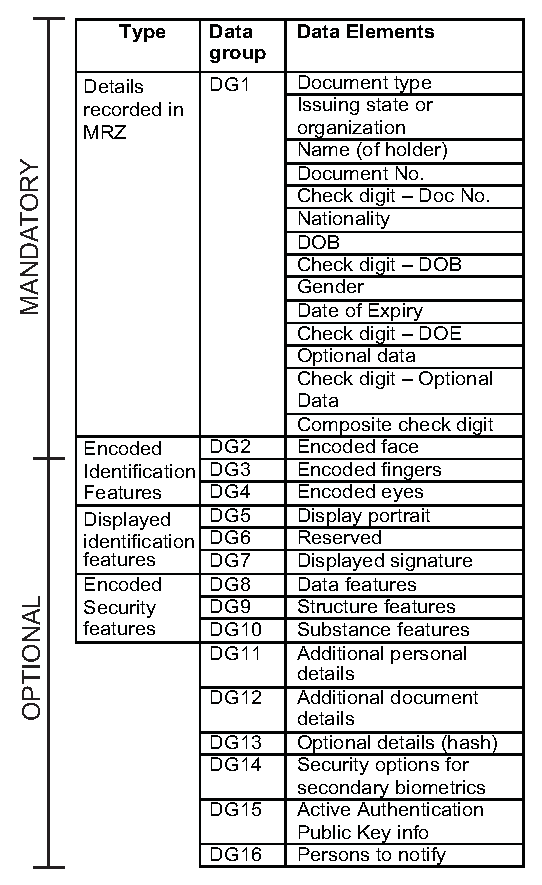
\includegraphics[width=4in]{LDS.eps}
\caption{The Logical Data Structure required to be ICAO compliant \cite{Anonymous:2006vu}}
\label{fig:LDS}
\end{figure}

\section{Implementation}
{\color{red}{This section could cover practical issues related to the implementation of an algorithm, protocol, or system, and may link to demonstration software that has been developed as part of the project.}}

The security of the ePassport must be secure in both directions. The reader of the data held within the ePassport wishes to verify the integrity of the data, effectively to be sure that the holder of the passport is who they say they are. The Passive Authentication (PA) protocol in combination with Active Authentication (AA) protocol, or the proposed Chip Authentication (PA) protocol ensures this integrity.

On the other hand, the holder of the ePassport does not wish to provide its sensitive data to an unauthorised source, currently there is no mandatory protection of this data, however the Basic Access Control (BAC) protocol has been widely adopted. BAC as we shall shortly discuss is not as secure as it was initially believed and is thus not recommended for protecting sensitive biometric data. A new protocol, EAC, has been proposed for this purpose. As we shall discuss this protocol in its newest state overcomes many of the problems with the BAC and it is likely to be adopted by the next generation of ePassports.

We will now discuss these technologies in depth. We will consider how the protocols work in conjunction with public-key cryptography and digital signatures to maintain a secure system maintaining data integrity and authenticity of the data.  

\subsection{Passive Authentication (PA)}
\label{sec:PA}
Passive authentication is a method of ensuring the data integrity of the information on the ePassport. PA is a system where by the data stored in the data groups is hashed using a hashing function, often SHA-1 \cite{Avoine:2008wf}, forming a checksum of the data held. 

\begin{figure}
\centering
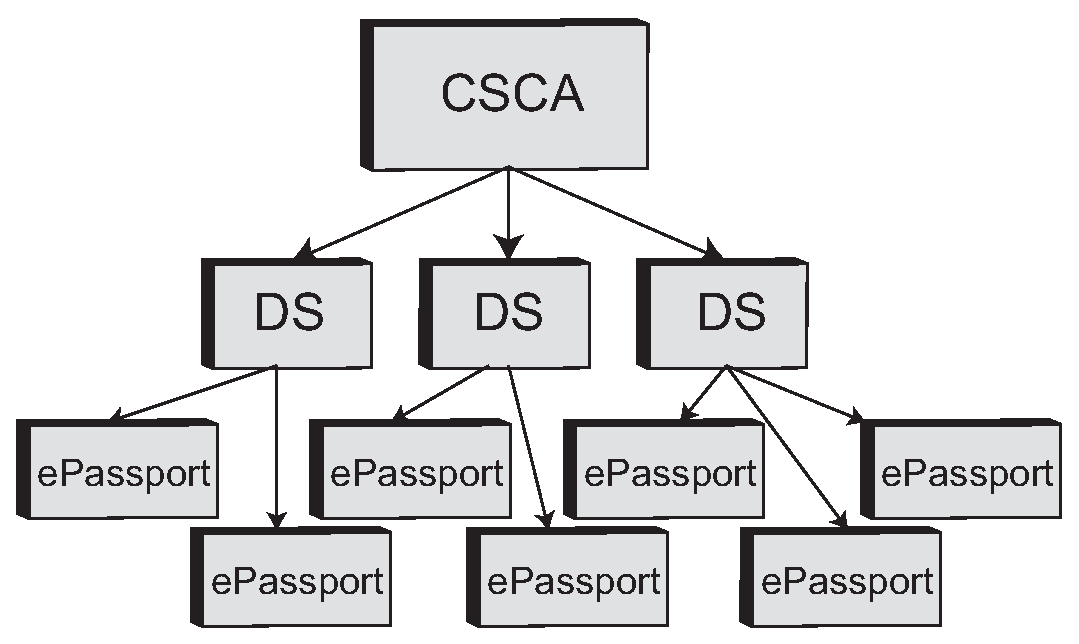
\includegraphics[width=4in]{IACO-PKI.eps}
\caption{ICAO-PKI}
\label{fig:ICAO-PKI}
\end{figure}

The PA implements a PKI (Section~\ref{sec:PKI}) hierarchy with a two levels of authority (Figure~\ref{fig:ICAO-PKI}). A Country Signing Certificate Authority (CSCA) is designated for each country. The CSCA in turn designates a variety of Document Signers, who are bodies responsible for issuing passports \cite{Anonymous:2011vj}. In the personalization phase of the ePassport the certificate produced by the Document Signer (DSC) is added to the ePassport, which are in turn signed for their authenticity by the CSCA's private key. The DSC is also held in a Public Key Directory (PKD) hosted by ICAO (Figure~\ref{fig:PKD}), which provides all countries access to a list of Document Signer Certificates. This Document Signer Certificate is a signature promising the authenticity of the passport being produced and is thus trust in this signature is central to the verification of the ePassport. The Document Signer Certificate carries the Document Signer Public Key (DSPuK). Anyone who holds the DSPuK can decode any messages encrypted by the Document Signer Private Key (DSPrK).

\begin{figure}
\centering
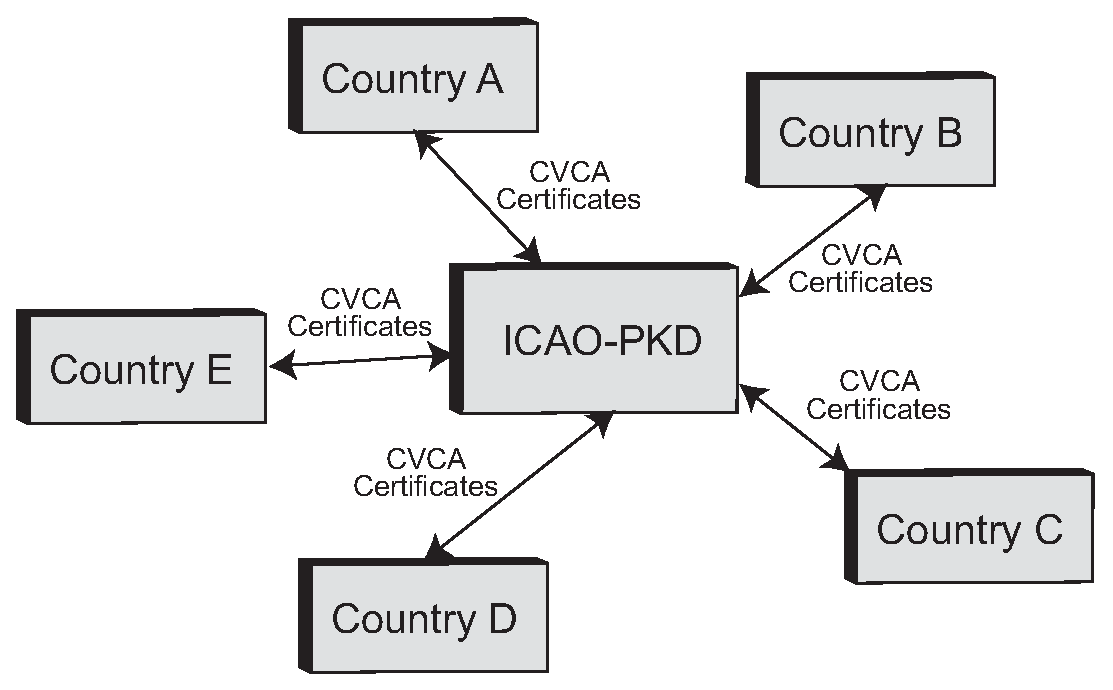
\includegraphics[width=4in]{ICAO-PKD.eps}
\caption{ICAO-PKD}
\label{fig:PKD}
\end{figure}

The hash of the contents of the is signed by the Document Signer Private Key and stored in a file called the Document Security Object (DSO), which can in turn be decoded by anyone in possession of the Document Signer Public Key. Although the DSPuK is public knowledge (distributed openly by the ICAO) it ensures that nothing has been changed in the encoded message, if it had, the resulting hash which had been decrypted, would be different from the hash that was initially signed by the DSPuK.

The Inspection System (IS), the terminal attempting to read the data, is responsible for checking the hash of the data still matches that of the data held in the Document Security Object (DSO). It does this by decoding the DSO using the Document Signer Public Key, either held in IS itself (or accessible from the PKD), or held in the DSC of the ePassport. When the hash is recovered, it computes its own hashes of the contents of the Data Groups. If the two hashes do not match exactly, the data in the Data Group has been tampered with and cannot be trusted, if they match, it is extremely likely that they are identical (see Section~\ref{sec:hashing} for details) and thus can be trusted. 

The problem with Passive Authentication is that although makes it extremely difficult to change data held within the chip without it being immediately obvious to the Inspection System, it does not protect against the chip in the ePassport being cloned. If all of the data of the chip were copied bit to bit to another chip, there would be no way of the Inspection System knowing the difference between the two ePassports. 
Another very avoidable problem is that if countries are not using the ICAO PKD to gather their Document Signers Certificates, and are instead assuming that the DSPuK held in the chip are valid, it would be easy to forge the signature as a `new country' \cite{ePassportsreloaded:2009ti}.

\section{Active Authentication (AA)}
\label{sec:AA}
Active authentication attempts to overcome the shortcomings of Passive Authentication by ensuring that the ePassports chip cannot be copied or forged and still passes itself off as authentic. Currently, and worryingly, this is not a requirement for any state issuing ePassports. It is actually only used by a small number of countries, in 2009 only 20\% \cite{ePassportsreloaded:2009ti}.

The authentication works again by capitalizing on public-key cryptography. Here a public and private key is created specifically for the chip being used, known as the Active Authentication Key pair (AAPuK and AAPrK). ICAO \cite{Anonymous:2006vu} states that a hash of the public group info held in DG15 is additionally stored in the DSO previously discussed in Passive Authentication (Section~\ref{sec:PA}). The Document Signer who issued the passport as previously described signs this. The effectiveness of Active Authentication revolves around the security of the private key; it should be impossible to copy this from the chip. To ensure that this private key cannot be copied the key is held in a secure memory area of the chip. Passive Authentication has already verified the integrity of the data at the point of Active Authentication. At the point of AA, we know for sure that the AAPuK is valid; we now wish to check that the corresponding AAPrK is present on the device to verify the chips authenticity (as the AAPrK cannot have been duplicated).

\begin{figure}
\centering
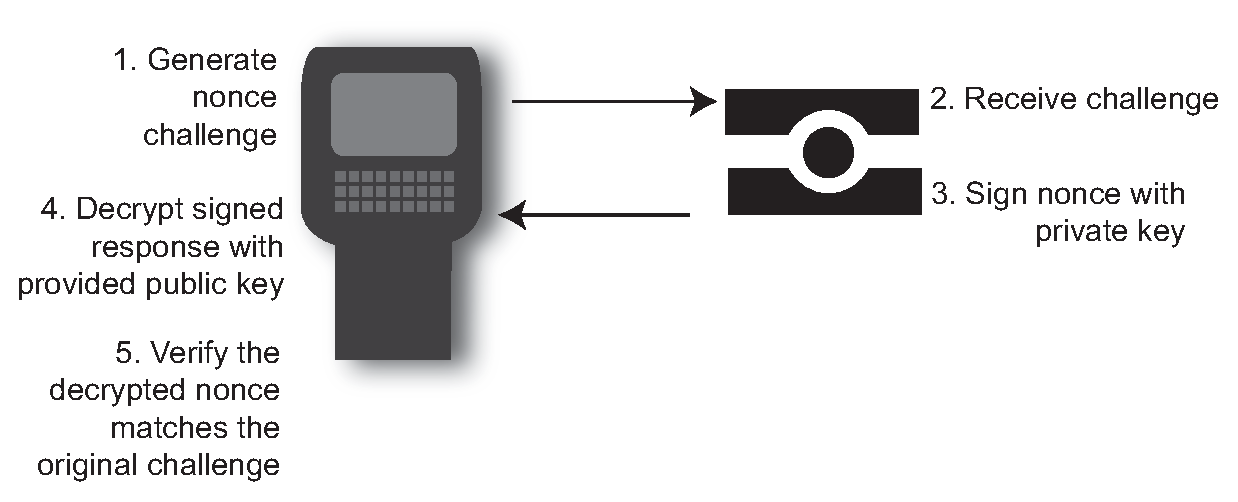
\includegraphics[width=5.5in]{AA-Challenge-Response.eps}
\caption{Challenge-Response protocol utilised by Active Authentication (AA)}
\label{fig:AA}
\end{figure}

The protocol is a simple challenge-response protocol (illustrated in Figure~\ref{fig:AA}). It begins by the Inspection System generating a nonce (a new random number) and challenging the chip to sign it with its AAPrK. The chip signs the nonce with the AAPrK and passes the resulting encrypted nonce to the IS. The IS in turn uses the verified AAPuK read from the chip to decrypt the nonce and checks that it is identical to the nonce initially passed. If the chip was a forgery, it would not contain the matching AAPrK to the AAPuK stored in DG15, and as such it would not be able to encode the nonce in a way could be decoded by AAPuK. 

When implemented properly this method of authenticity verification is believed to be very effective. However, various hacks have been discovered to both disable the Active Authentication checking (which has been fixed in recent Inspection Systems software), and also recovering the AAPrK through power analysis when a challenge is made \cite{Witteman:2005ta}. The latter hack has more drastic consequences, as if a chip can be made with an identical copy of all the chip data, and the AAPrK was to be saved to the secure memory area of the chip, they the passport chip would appear indistinguishable from the authentic chip.

\section{Basic Access Control (BAC)}
\label{sec:BAC}
So far we have only discussed the inner workings of mechanisms designed to ensure data integrity and authenticity, we will now look at methods by which read access is authorized for the sensitive material held on the ePassports chip. Although to be ICAO compliant it is not required to defend the chip from unauthorized reading, at least some protection has been provided by almost all states using ePassports \cite{Chothia:2010wf}.

The aim of BAC is to agree on a key with which messages between the Inspection System and chip can be encrypted. It also attempts to evade attacks that do not try and learn the information encrypted, but attempt to replay previous conversations. For example an attacker may wish to replay an authorization request to initiate a session.

The implementation of BAC relies on strong conventional symmetric encryption techniques such as 3DES (Section~\ref{sec:3DES}) to secure a conversation between the Inspection System and the chip, where messages can be trusted they are from a secure source. The chip holds two keys, denoted KE and KM. These keys can be derived from the Machine Readable Zone (MRZ) of the passport, which is a long string located on the page of the passport usually located on the same page as the biometric facial image. The fact that this string is required is central to the security of BAC, and as we shall discuss momentarily, is one of its major flaws. The Inspection System is expected to read the string in the MRZ (often using OCR) and derive the keys KE and KM in order to initiate the conversation with the chip.

Once the keys KE and KM have been derived, the IS sends a challenge to the chip of the ePassport. In response the chip generates a 64 bit nonce, NC, which is passed back to the IS. This nonce ensures that the conversation cannot be replayed to the chip, as each conversation is unique. The IS then generates its own random nonce NIS and 64 bit key KIS. NC, NIS and KIS are then encrypted by the 3DES (for the UK, other countries agree on their own encryption algorithms) algorithm using the KE key derived from the MRZ, this message is denoted EN. Additionally a checksum (SHA-1 hash - known as MAC) of the encrypted message is encrypted by KM and sent as a message denoted MN. The MN acts similarly to the digital signature used in Passive Authentication, confirming that EN has not been modified. However, whereas a digital signature is signed with a private key, MN is signed with a shared key KM. The process of encoding messages and MAC's is illustrated in Figure~\ref{fig:MACencoding}.

\begin{figure}
\centering
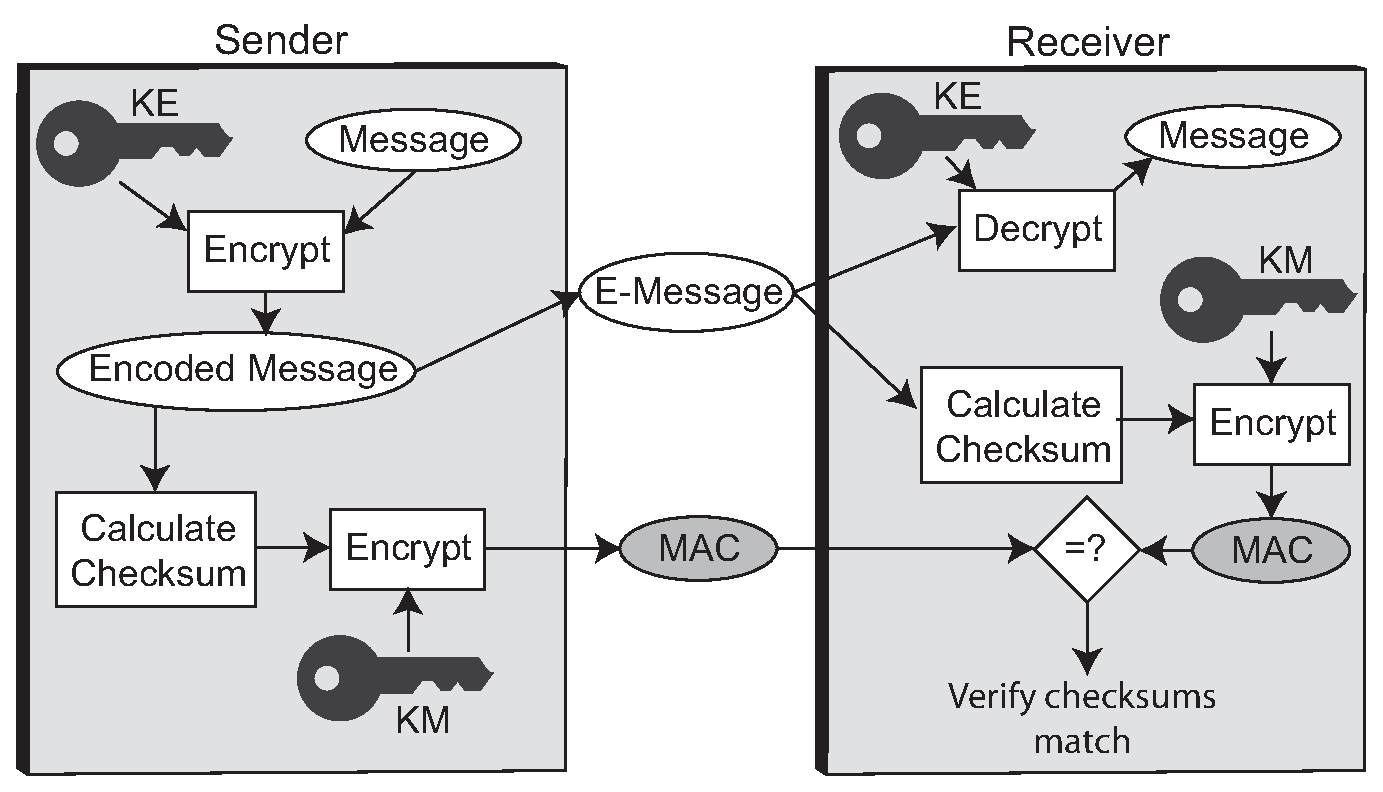
\includegraphics[width=5.5in]{MAC.eps}
\caption{Encoding and decoding with shared keys and MAC verification, KM is the MAC key, KE is the encoding key.}
\label{fig:MACencoding}
\end{figure}

Both messages are then sent back to the chip. The chip decrypts the messages using KE and KM that are stored within its memory. If the decrypted NC from EN does not match the one sent, authorization is refused based on mismatching nonces. If checksum held within the MN message does not match the SHA-1 hash of the message held in the decrypted EN, authorization is refused on the grounds of mismatching MAC. If both the hash and the nonce match, then the chip generates a new string KC. The new key is combined with the two nonces (however their order is reversed to avoid playback of the message). This message is again 3DES encrypted with the key KE, and an encrypted checksum (MAC) is sent encrypted with key KM. 

Finally the Inspection system decodes the messages and verifies that the nonces match and the MAC matches. Both the inspection system and the chip have now securely passed one another their preferred random key. A key that can be used to encrypt the remainder of the conversation is obtained simply by performing an XOR between the two keys (KIS and KC) and denoted as KSEED \cite{Chothia:2010wf}.
 

Despite this apparently very secure transmission of keys and nonces the system is known to retain some flaws that have been discovered by security experts since their introduction. Many sources \cite{Juels:2005wf, Avoine:2008wf} have commented on the relatively low entropy of the MRZ string required to derive the keys required for communication. Some countries such as Belgium use a MRZ string with entropy as low as 38 bits, and if the attacker has knowledge of the victim's date of birth, down to 23.

As \cite{Hoepman:2006tg} noted, ECRYPT EU Network of Excellence on cryptology recommends minimum entropy of 80 bits for general-purpose protection (in 2005) and 112 bits from 2015. With an entropy as low as 23, an attack to derive the key to be used for BAC would take less than one second on any modern machine \cite{Avoine:2008wf}, making skimming a viable concern. A table of other countries respective entropies can be seen in Table~\ref{tab:MRZ-entropy}.

\begin{table}
    \centering
    \begin{tabular}{|c|c|c|}
        \hline
        Country&Effective&Birth date known\\
        \hline
        Germany&55&40\\
        \hline
        USA&54&39\\
        \hline
        Netherlands&50&35\\
        \hline
        Belgium&38&23\\
        \hline
        Spain&51&36\\
        \hline
        Italy&51&36\\
        \hline
        France&52&37\\
        \hline
    \end{tabular}
    \caption{Countries ePassports MRZ entropy. Compiled from \cite{deladefencenationale:2008wf, Avoine:2008wf}}
    \label{tab:MRZ-entropy}
\end{table}

Another concern raised by Chothia et al.\ \cite{Chothia:2010wf} arises from the incomplete implementation specifications. Each country implements their own version of the BAC protocol, and as expected this results in inconsistencies. Chothia developed a hack (code can be found at \cite{ChothiaPassportAtt:wz}) that capitalizes on such an inconsistency to allow any e-Passport to be tracked without the holder's knowledge. The hack uses the fact that some BAC implementations return different errors when the authentication fails due to mismatching nonce's, to authentication failure due to mismatching MAC.

A valid conversation been an inspection system and an ePassport can be recorded (since RFID is contactless, these communications can be recorded from a few meters away). If this message is replayed to the same ePassport it will validate that the message is indeed correct, except that it isn't using the random nonce it told the inspection system to encode. As such it will reject the authentication based on mismatching nonce's. If the same message was replayed to a different ePassport, the MAC would not match and authentication would be rejected on the bases of a mismatching MAC.

Armed with this knowledge, an attacker than then set up systems wherever he wishes which probe all passports with recorded messages, and logging whether authorization was rejected on the basis of incorrect nonce or MAC. The attacker will then know whether an individual has passed their probe at any point in time. This type of attack is known as a traceability attack. Although many ePassport holders do not keep their passport on their persons at all times, with the possible introduction of identity cards using similar technology this type of attack is a cause of concern.

\section{Extended Access Control (EAC)}
\label{sec:EAC}
BAC provides loose protection of the ePassports biometric data from skimming and eavesdropping. The protection provided is based on an assumption that an attacker cannot gain access to the MRZ, printed on the inside of the passport. Much of the data held in the LDS is already encoded in the MRZ, as such if someone has access to the MRZ, they can easily decode the information held in DG1 and DG2. 

The Extended Access Control (EAC) protocol provides more extensive protection for more sensitive biometric data such as the fingerprint and iris scans and additional information held in DG3-DG14. The protocol wishes to authenticate that even if the passport is in the possession of someone, they cannot necessarily read all the sensitive information held within.

The security of EAC can be broken into two components, Terminal Authentication to verify the inspection system is authorised to read sensitive data, and Chip Authentication that furthers the ability to authenticate that the chip is valid, and serves as a updated replacement for Active Authentication (Section~\ref{sec:AA}).

\subsection{Terminal Authentication}
\label{sec:TA}
Terminal authentication ensures unauthorised readers cannot read private data. The authentication uses asymmetric encryption to ensure this.

The protocol requires that each country involved implement their own three-layer PKI (Figure~\ref{fig:EAC}). Each country, similarly to Passive Authentication (Section~\ref{sec:PA}), appoints their own nationally trusted anchor, called the Country Verifying Certification Authority (CVCA) as the root of their PKI. In the second layer there are many Document Verifier Certification Authority (DVCA). DVCA's possess certificates from any countries willing to allow the DVCA to issue Inspection Systems (IS) the authority to read sensitive biometric data held on the ePassport such as fingerprint and iris scans. Finally, DVCA's issue certificates to IS's that wish to read the sensitive data, a certificate is provided for each country the inspection system is authorised to read from. This is a certificate chain, each IS will hold a certificate chain where each certificate is signed by an overlooking authority.

\begin{figure}
\centering
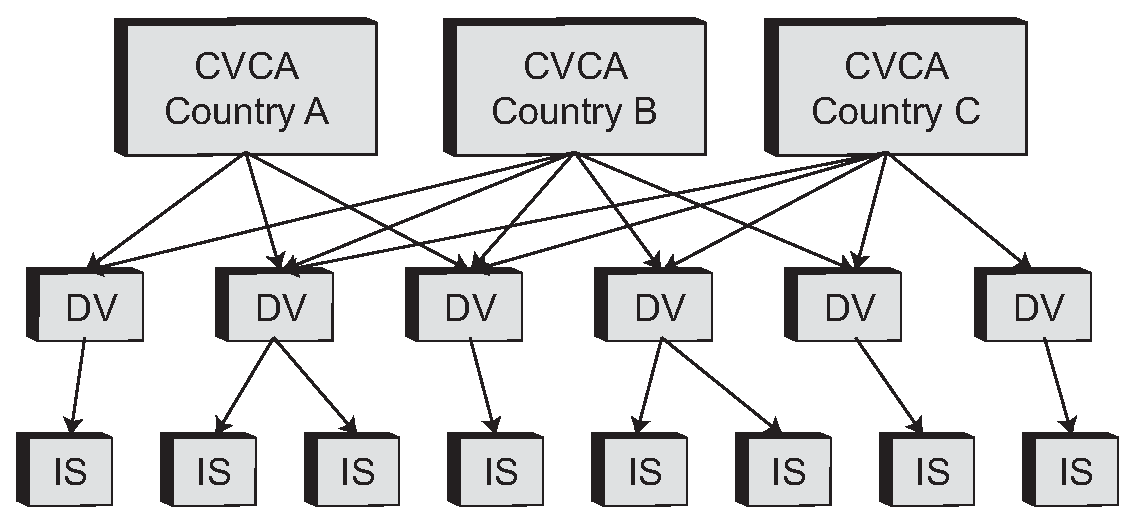
\includegraphics[width=4in]{EU-EAC.eps}
\caption{PKI to be implemented by each country compliant with ICAO EAC protocols. Here a Inspection System (IS) in Country C cannot read the sensitive data of a ePassport issued by Country A.}
\label{fig:EAC}
\end{figure}

As with many PKI's each certificate possesses its own validity date. Within the specification of PKI's required for EAC authentication, each layer down should have a smaller validity window, thus if a inspection system is compromised, it will only possess the ability to read sensitive data for a couple of days. Keeping relatively short validity periods avoids the needs for a Certificate Revocation List (CRL) typically used in PKI's for when a component is compromised.

Each ePassport chip can verify the certificate chain (illustrated in Figure~\ref{fig:cert-chain}). It will first decode the message using the public key held in the IS certificate. The chip then needs to check that this certificate indicates that the IS is authorised to read the secondary data. This can be verified by reading the DV certificate issued by the DVCA to the IS, sent within the certificate chain. If the DV certificate is digitally signed by the CVCA of the ePassport's issuing country, the DVCA was authorised to access the sensitive information, and in turn is authorised to allow the IS to access the same information. This can be checked as the ePassport contains the root CVCA certificate of its country of issuance, thus knows the public key for the top level of the certificate chain. If the IS does not hold a DV certificate signed by the ePassport's CVCA, then authentication should be rejected.

Once the chain has been fully verified that it authorises the owner of the certificate to access the secondary data, the protocol must check that the certificate belongs to the IS asking for the data. The public key sent with the certificate allows this check to be made. If the IS has the corresponding private key the certificate belongs to the IS. A challenge-response protocol ensures that the IS has the private key. The IS requests a challenge, followed by a random nonce response from the chip. The IS encrypts the nonce with the private key and returns it to the chip, if the chip decodes the encoded nonce with the public key provided, the IS must be in possession of the corresponding private key.

\begin{figure}
\centering
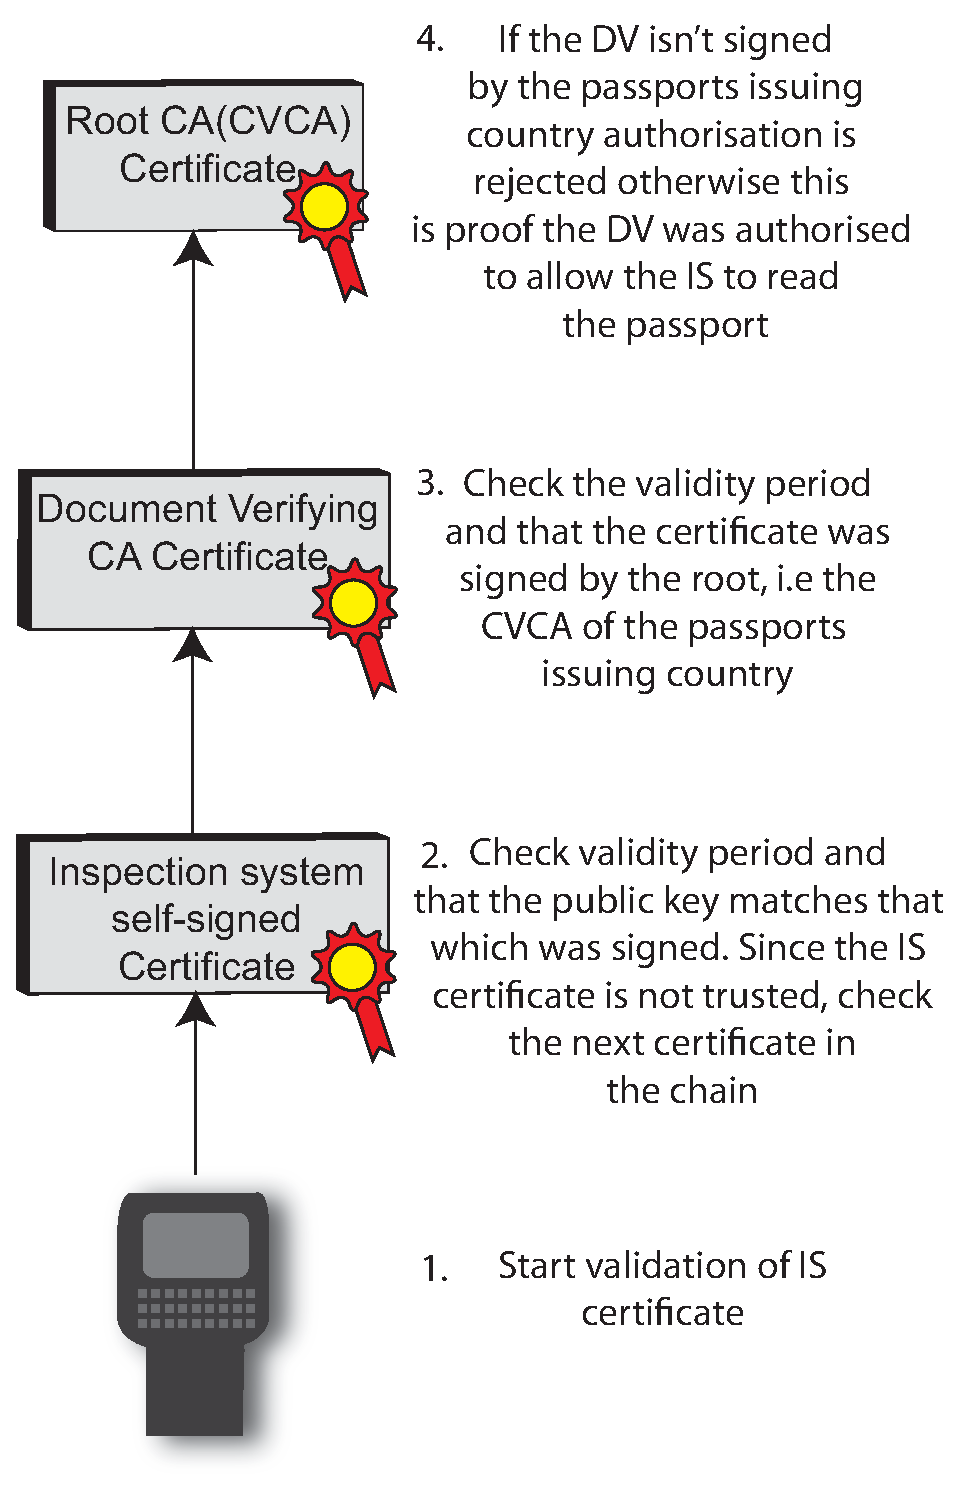
\includegraphics[width=4in]{Certificate-Chain.eps}
\caption{Certificate chain being checked during Terminal Authentication (TA). Inspired by \cite{OracleCertificateC:wr}.}
\label{fig:cert-chain}
\end{figure}

This provides a very high level of security, however as Chaabouni et al.\ \cite{Chaabouni:2008wb} notes, ICAO states in their specification for the EAC protection that less sensitive data should be accessible via BAC. As such, even though the protection methods exist for keeping all of the passport holder's data, information such as name, date of birth, passport number and a biometric image of the face, must be obtainable through a far less secure protocol. 

There are several further vulnerabilities of the EAC protocol as noted by Pasupathinathan et al.\ \cite{Pasupathinathan:2008vy}. A weakness with the use of current generation of RFID is that there is no internal clock. In order to verify that a certificate has not expired the chip needs an estimate of the current time. The EAC protocol states that this estimate should come from the time at which the last acceptance during certification verification occurred. The chip initially has its current date set to the date at which the CVCA certificate was issued. Persons who travel infrequently may have their time estimate out by a matter of months. Verification of the expiry date simply consists of the chip checking that the expiry date is posterior to the current estimate of the date. 
Since IS's certificates expire significantly more quickly than that of the CVCA, it is easy to see how a compromised IS may still be authorised for a significant amount of time after its expiry date.

Another security concern arises from the same requirement of an internal clock. Since the clock must be updated, parts of the chip now must contain writable partitions that the previous generation did not contain. ICAO does not specify a required method of securing this area. If an attack could modify the current time to a date significantly in the future, then the ePassport would become unusable as all certificate expiry dates would be prior to the believed current date. Indeed Luks Grunwald demonstrated this hack in 2007 \cite{SecuritybyPolitics:2007uh}.


\subsection{Chip Authentication (CA)}
\label{sec:CA}
The Chip Authentication (CA) protocol is an improved replacement for Active Authentication (Section~\ref{sec:AA}). Its purpose is to ensure that the ePassports chip is authentic and has not been duplicated or copied. It provides both an authentication of the chip of the ePassport and generation of a session key for further communication \cite{Pasupathinathan:2008vy}.
The protocol is started once a conversation has been established using the BAC protocol. It utilizes the Elliptic Curve Diffie-Hellman (ECDH) \cite{Menezes:1993ua} to generate a more secure communication channel. 
The public key AAPuK that was used in the previous method of authentication - Active Authentication - is sent along with its domain parameters, DC, to the Inspection System (IS). The IS then generates a temporary ephemeral key pair using the domain parameters and passes its public key to the chip. It is then possible for both the chip and the IS to generate a shared secret from the public key and the domain parameters by simply multiplying the by their private key due to elliptic curve cryptography. 
The shared secret is used to derive two session keys, KM and KE for the MAC and encoded respectively. The nonce and an authentication token composed of KM and it's public key are sent to the IS. The IS derives the same session keys KM and KE using the shared secret and the random nonce and verifies the authentication token matches. These session keys can then be used for further 3DES encrypted secure messaging \cite{derInformationstechnik:2012ta}.

Since the shared secret could not be derived without possessing the corresponding private key to the public key disclosed, this method ensures that the chip holds the private key, thus performing the same action as Active Authentication, whilst also ensuring that a strong key is used. Since the cryptographically weak BAC protocol was previously used to derive the key for secure messaging up until this point, it is important to ensure that the key used in sharing sensitive information is changed.

It is important to verify that the public key belongs to the chip; as such passive authentication must be performed immediately after this exchange. This ensures that the public key shared by the chip has not been tampered with (See Section~\ref{sec:PA} for details). 
Although this protocol improves on Active Authentication in the respect of generating a secure messaging key after initial authorization is given, it still suffers from channel attacks whereby the private key held in the unreadable memory can be obtained by power analysis \cite{Blundo:2008uf}.


\section{Password Authenticated Connection Establishment (PACE)}
\label{sec:PACE}
The Password Authenticated Connection Establishment protocol aims to overcome some of the shortcomings of BAC. BAC determines the secure messaging protocol key using purely the MRZ causing low entropy keys, KN and KM. PACE creates a high entropy key from a low entropy passport. The password used for this key creation can come from either a Card Access Number (CAN) or a MRZ, both of which are short. The CAN could either be statically printed on the same page the MRZ is on, or it could be dynamically created and displayed using low power display technology such as OLED \cite{Nithyanand:2009ud}. Given this shared password has been read and is known by both the IS and the chip being read, a Diffie-Hellman key exchange can be used to create keys for encryption, KN and KM.

The chip first generates a random nonce. This is encrypted by a key composed of the hash of the password. The encrypted key is then sent to the IS along with a set of domain parameters that will be used in constructing a public/private key pair. The IS receives the encrypted nonce and decrypts it using the shared password. The IS and chip generate their own unique Diffie-Hellman temporary key using the domain parameters and nonce shared between them. The public keys are shared and both generate a shared key as in Chip Authentication (Section~\ref{sec:CA}). This shared key is used to generate the session keys used in secure messaging, KN and KM.

The Federal Office for Information Security (BSI) introduced this protocol in 2008 along with updates to EAC protocols CA and TA \cite{Nithyanand:2009ud}. This protocol along with EAC overcomes many of the most serious concerns experts have with the security of our national passports. By dynamically creating shared passwords, the BSI would be taking a leaf from the new age financial security whereby new passwords are given for each individual session which need to be physically entered before any communication can begin.

\section{Data and evidence}
{\color{red}{A strong report will make good use of data that are either collected as part of the project (please stay within the legal framework - so don't collect  data  on  system  vulnerabilities!),  or  publicly  available,  as  well  as  other published material.
Blah}}

\section{Discussion}
{\color{red}{This section will set the findings of the report within a wider context, and may for example make a case for including this material as part of the lectures in the module next year.}}

We have surveyed the current authentication, verification and encryption methods and protocols used in past and current generation of ePassports. 
A theme frequently seen in security applications has arisen of apparently solid protocols being developed and concerned and interested experimentalists and enthusiasts somewhat successfully proving how weak they are.

It is clear as we move further into the technological age that we are making more and more information about ourselves publicly available. However, many find it disconcerting how information we do not wish to share can be extracted against our will. Passports are prime candidate for such exploitation. Passports contain some of the most important details defining our identity in the legal world, and are trusted almost unconditionally when provided. 

We have shown in this report how although the security behind the relatively new technology of ePassport chips has improved, it is still a significant weakness in protecting our identity from threats such as identity theft. Many security and RFID experts such as Luks Grunwald are extremely vocal and open about their concerns, even demonstrating their weaknesses. 

An implication of implementing digital security within passports is that the field of cryptology moves relatively quickly, weaknesses in existing security protocols are uncovered year on year, however in the digital domain often the applications relying on these protocols can be updated quickly to overcome these weaknesses. In contrast current adults UK passports are issued for up to 10 years without any need for renewal. At the high cost of replacement this cannot change easily. Considering the BAC protocol was shown to have flaws within 48 hours following its introduction in 2005 \cite{Crackedit:wc}, basic flaws will remain to be a problem for long after their weaknesses are discovered. 

Hacks have been discovered that provide the ability for passports to be traced (Section~\ref{sec:BAC}). The government are already conscious of a growing concern over privacy concerns. With the proposed introduction of Identity cards in countries such as UK \cite{JRC:2008ws} holding sensitive fingerprint information and using very similar protection protocols this concern is only likely to rise. Such ID cards are already in operational in Spain and Portugal. Germany is also planning to produce a centralised database of fingerprints for all of its nationals. Many are concerned as this allows for the introduction of an ``Orwellian Nightmare".

There are campaigns for the abolishment of RFID tags supported by some of the most important computer scientists of our age such as Richard Stallman who are concerned with the privacy implications.

We hope that this survey has opened your eyes to not just the technical details of the protocols used, but its flaws and implications on our modern society.
\cleardoublepage
%\addcontentsline{toc}{chapter}{Bibliography}
\bibliography{mybib}
\bibliographystyle{plain}
 
\newpage
Useful bits:

PKI:
http://www.jrpit.acs.org.au/jrpit/JRPITVolumes/JRPIT40/JRPIT40.3.187.pdf

EAC:
{\color{red}{
Maybe try make an implementation of a simple PKI with python?

For comparing v1 v2 etc:
http://eprint.iacr.org/2010/103.pdf

For overview of PKI authentication method
http://www.cryptomathic.com/media/12100/cryptomathic\%20cvca-dvca\%20product\%20sheet.pdf 

Paper with EAC description, CA and TA, and vulnerabilities!
http://www.springerlink.com/content/n478131u3xv35062/fulltext.pdf 

Diagrams
http://www.cryptomathic.com/media/12100/cryptomathic\%20cvca-dvca\%20product\%20sheet.pdf
http://www.secunet.com/fileadmin/user\_upload/Download/Printmaterial/Factsheets/englisch/sn\_eID-PKI-Suite\_FS\_E.pdf	
http://www.jrpit.acs.org.au/jrpit/JRPITVolumes/JRPIT40/JRPIT40.3.187.pdf
}}


CA:
{\color{red}{http://www.informatik.tu-darmstadt.de/fileadmin/user\_upload/Group\_TRUST/PubsPDF/BPSV08.pdf
https://www.bsi.bund.de/EN/Topics/ElectrIDDocuments/SecurityMechanisms/securEAC/securCA/ca\_node.html}}

Discussion:
{\color{red}{Provides information on which countries have what on their passports/ID cards
http://ftp.jrc.es/EURdoc/JRC48622.pdf}}

LDS:
{\color{red}{Image - maybe steal the figure from: E-Passports as a Means Towards the First World-Wide Public Key Infrastructure}}

\end{document}  
